\documentclass[a4paper,12pt,titlepage]{article}
\usepackage{geometry}       % allows changing page dimensions
\geometry{a4paper,left=2cm,right=2cm,top=2.5cm,bottom=2cm}
\usepackage[latin1]{inputenc}   % support the pt encoding
\usepackage{graphicx}       % support graphic files
\usepackage{color}          % should allow colored text
\usepackage{url}            % should identify and format urls
\usepackage{natbib}         % pretty bibtex
\usepackage{enumerate}			% allows enumerations a)... I..., 1... etc.
\usepackage{rotating}				% allows text rotate via \begin{sideways} or \begin{turn}{ang_in_deg}
\usepackage{lscape}					% allows pages in landspace \begin{landscape}page content\end{landscape}

%\def\hellow{
%	\textcolor{red}{HELLO!}
%}
%
%% with receiving param
%\def\hellow2#1{
%	\textcolor{red}{begin #1 end}
%}
%
%% alternative way of starting ending a command
%\def\hellow3#1{
%	{\bf#1}
%	\begin{bf}#1\end{bf}
%}

% show TODOs
\def\TODO#1{
	%\glossary{#1}
	\textcolor{red}{\textbf{TODO:} #1}
}

% hide TODOs
%\def\TODO#1{}


% LANGUAGE PROBLEMS:
% too much the's and a's
% too long sentences, use commas
% write in the third person singular

% TACTICS:
% get articles from gdx techniques such as raytrace, bsp, radiosity, etc.

%
% TODO
% - ABSTRACT
%   good
% - INTRODUCTION
%   ok
% - PROBLEM
%   done, not too cool
% - APPROACHES
%   67%
% - COMPARATIVE ANALYSIS
%   0%
% - CONCLUSIONS
%   0%
% - add comparative table
% - IST logo @ title page

%\title{\textsc{Survey}\\\textbf{creating urban scenery\\using multimodal interfaces}}
\title{\textsc{Survey}\\\textbf{creating urban scenery\\using multimodal interfaces}\\\textcolor{red}{\small{DRAFT from \today}}}
\author{\textbf{Jos� Pedro Dias}\\n.48296\\\emph{jose.pedro.dias@gmail.com}}
\date{January 2007}

\makeindex
%\makeglossary

\begin{document}

\maketitle
%\newpage

\tableofcontents
%\listoffigures
%\listoftables
\newpage

%\twocolumn
	
\baselineskip = 16pt    % bigger space between lines

\section*{Abstract}
\chapter*{Abstract}
\addcontentsline{toc}{chapter}{Abstract}

\TODO{review and summarize this part, add implementation part.}

% context and problem
Nowadays the architectural project workflow is highly segmented
between the creative part and the CAD modeling part.
It starts with the architects drafting hand-made sketches of building designs
to study viable designs and validating them with clients, a stage without computer usage, 
with all participants on location using pen and paper.
Later on a set of documents is generated from the ground up on CAD software, 
using desktop computers and WIMP interfaces.

% motivation, goals
There's an increasing availability of alternative methods for both sketching, navigation and visualization
of 3D scenes which can enrich the design process and provide a better experience for both
building drafting, visualization and review.
We're committed to developing a multimodal distributed system to fulfill these goals
using tablet PCs or other devices facing a powerwall.
%We're committed to developing a multimodal system allowing multi-user scene navigation,
%building draft building designs, navigation and content reviewing.
It is thought out to integrate the architectural workflow as a creative and reviewing tool
to complement the early stages of architectural design.

% document organization
This survey begins with an analysis of projects with similar goals,
followed by a set of issues to handle:
how to get input from users,
display interactive content to them,
make shape creation and transformation possible and
allow scene navigation
%provide content reviewing capabilities.
A comparative analysis between architecture creation systems available in the market is then conducted and
finally conclusions are reached and directions for project execution defined.

\textbf{Keywords:} urban architecture, city, building, multimodal interaction, navigation, content reviewing


%\newpage

\section{Introduction}
% Context + Problem

% http://en.wikipedia.org/wiki/Architecture

\subsection{The Evolution of Architecture}
Architecture is the art and science of designing buildings and structures.
It is an interdisciplinary field which has similarities to applied science and
engineering, but unlike them, focusing on functional and feasibility aspects of design, 
architecture deals with building costs, space and volume, materials and lighting
in order to achieve an aesthetically pleasing result.

For centuries methods and norms have arisen. Architects tools of work were based on paper and ruler.
With the evolution of computational power throughout the last century, 
increasingly more complete, fast and robust Computer Aided Design (CAD) systems were developed and so did
devices capable of manipulating architectural entities -- such as the mouse, trackball, tablet, etc.

\subsection{Current Workflow for Building Design}
% only geographical, drawings?
Elaborating architectural designs usually starts by drawing rough sketches of the subject
in order to convey form, proportion and lighting.
Relevant geographical data about the location where the building is to be established is acquired.
A series of two dimensional drawings is created in order to precisely define building features, dimensions and location.
These drawings serve as input for civil engineers and the rest of staff responsible for constructing the building.
Three dimensional drawings and brochures are created and scale models are built,
allowing people with no architectural background to better perceive the building before it is built.

Nowadays architecture is slowly but steadily embracing usage of computers in the designing process.
Authoring systems such as Autodesk's AutoCAD
\cite{SITE-AUTOCAD}
are currently used to produce a set of views and floor plans necessary to construct a building.
These systems are optimized for such tasks, having limited support for general 3D volume and surface creation
and rely heavily in desktop interfaces with keyboard/mouse.

The creation of 3D drawings and brochures for marketing purposes is common practice.
It relies in techniques such as
ray tracing \cite{SITE-POVRAY},
radiosity,
physically accurate light simulation \cite{SITE-MAXWELL}, \cite{SITE-INDIGO}; 
High Dynamic Range Imaging (HDRI), etc.
These techniques produce believable results but take too much time to render in real time.

% articles for bsps, octtrees, light rendering alg?
Another application for data coming from CAD systems is the generation of worlds optimized for navigation.
Performance is paramount in these systems so algorithms such space partition --
Binary Space Partitions (BSPs) for closed space rendering,
OctTrees for open space rendering --
and multiple Levels Of Detail (LOD) for each shape are commonly used.
The compromise between believability and fast rendering times is assured with techniques such as
light maps and using recent graphics card's Graphics Processing Unit (GPU),
shifting complex computer graphics algorithms out of the Central Processing Unit (CPU),
obtaining frame rates otherwise impossible with current hardware.

There are numerous 3D engines capable of presenting such worlds with good performance.
The major drawbacks in their usage rely on how the user navigates the scene --
most systems use the popular interface featured in most first or third person shooters,
relying on mouse/keyboard for input --
and on the lack of support for out-of-the-box interaction with shapes.
\TODO{UGLY PHRASE!}

\newpage
Exporting the geometry from a CAD program, which is a common solution, comes with several problems,
as stated by Alberto Raposo et al.\cite{CADVR06}:
\begin{description}
	\item[Low performance] -- due to unneeded model complexity;
	\item[Lack of realism] -- usually users of CAD programs don't associate material
	or texture data to objects;
	\item[Inadequate treatment of geometry] -- the conversion often occurs with loss of
	geometry, precision and errors such as badly oriented normals.
\end{description}

\subsection{Benefits and Goals of an Integrated Approach}
% client side benefits
Using a computer system to present a virtual building with the purpose of selling an idea,
doing real estate business or simulating virtual tours demands better metaphors,
better interface design and the least possible cluttering of the view in order
to achieve a richer user experience and get an overall good impression.
Navigating and reviewing content should be simple tasks to perform.

% architect benefits
From the architect's point of view, using such a system early in the process,
if preceded by geographical data capturing,
allows him to better perceive the construction area, which improves a seamless building integration.
Additionally, applying such a system in the building design workflow allows the generation
of models able to complement or even replace the first prototyping stages,
commonly represented nowadays by rough sketches.
The possibility of collaborative remote design and content reviewing offers a cheaper
alternative for distributed projects and allows a shorter validation cycle with the clients.

\subsection{Document Structure}
% structure for the rest of the document
This document continues with the identification of various problems that need to be solved in order
to fulfill these goals.
A series of projects in this area is then discussed.
Several subjects are then analyzed:
input modalities (using laser pointers, tablet PC pen, motion tracking and voice commands);
output modalities (using tablet PCs, powerwalls or head mounted displays);
shape creation and transformation (for modeling simple buildings, their translation, scaling, etc.);
scene navigation (using several modalities) and
content reviewing (by creating and editing shape attached annotations).
Later on a comparative analysis between applications in the market allowing architecture modeling is conducted.
The document ends with a set of conclusions and directions for future work in
addressing this subject.


\newpage

\section{The Problem}
% how and why to divide into these subproblems

% deliver?
We want to deliver a solution capable of being:
\begin{itemize}
	\item a sketch board for architects, who can create and edit buildings and their features;
	\item a virtual urban scenery for anyone -- therefore with gentle learning curve -- and suitable for showcasing and reviewing architectural designs.
\end{itemize}
In order to achieve these goals, there's a number of problems that need to be addressed.

% navigate in it?
% where -> at which?
One must be able to understand the world representation, navigate it and create or modify its contents.
In order to be immersed in the world, the interface should be larger than a regular computer screen,
in order for the users to better convey the proportions of the structural elements.
User input has to be based on devices that give him more expressiveness and allow human error,
preferably helping him out in subjects where a machine works better than humans do, such as figuring
out parallels or calculating areas.


% opensg/goggles/wall, etc
% city representations
\subsection{Representing Urban Scenery}
How can the system produce the most immersive experience for one user?
What if its a group of people? All this constrained by having to get user input at the same time.

How can we address the complexity of rendering a city?


% laser, motion, speech, gestures, smart widgets
\subsection{Getting User Input}
What are the viable alternatives to keyboard/mouse interaction with these objectives?
How can a user sketch his ideas, give orders, navigate? Should users move, point, talk?


% sketching
\subsection{Sketching for Geometry Creation and Editing}
Given sketching input, how can the system interpret the sketch and reason an object
out of it? Should the process be iterative or all in one step? How permissive should
it be to irregular shapes?
 

% by which?
% Helping the User: 
\subsection{Helping the User: Suggested Constraints}
There's a subset of geometry that appears quite often in buildings.
The walls are generally box shaped, as are most windows. We often use concepts of symmetry,
the golden ratio, equilateral triangles, spherical structures such as domes, etc.

It would be of great use if while sketching one could be aided in keeping the ratio of
a rectangle, draw parallel or perpendicular lines, do extrusions and lathes.

What are the available ways by which one could be aided in these tasks?


% navigation
\subsection{Navigation}
By what means should the user convey his position and orientation in the world?
What can he do and how? How to avoid users getting lost in the virtual world?



\newpage

\section{Approaches}
% group similar domain articles
% for every article write a short summary of its relevant features
% and add an illustrative picture
% then criticize the presented solutions

\subsection{Representing Urban Scenery}
In order to obtain an immersive experience, there's a number of hardware
setups commonly available:
\begin{description}
	\item[Head Mounted Display (HMD)] --
	  Head mounting displays are shaped like glasses. They normally feature a gyroscope or similar device
	  to measure head orientation and tilt.
	  
		Using a head mounted display has the benefit of sticking to the user's head and detecting head orientation.
		On the other hand each HMD serves one single user.
		Additionally most users report suffering from fatigue after long periods of usage and it has limited resolution.
	\item[Cave Automatic Virtual Environment (CAVE)] --
	  A CAVE is an immersive virtual reality environment where projectors are directed to four,
	  five or six of the walls of a room-sized cube.
	  
		Shares with HMDs the benefit of enclosing the user's viewing area.
		Has a better resolution though. The downside is the small number of simultaneous users who
		can experience the CAVE at the same time.
	\item[Wall] --
	  TODO
	  
		Its size and resolution depend entirely on the setup, but normally a wall offers high resolution
		(depends on the number of projectors in the grid and their resolution).
		The presence of a wall doesn't limit the number of users.
		The downside is that users have to face the wall!
\end{description}

Any of these setups is suitable for single user interaction.
In case of a reviewing session, in which at least two participants are required,
CAVE or Wall are better suited.

Using a Wall or CAVE presents other challenges: the computers responsible for
generating each projectors' images must be synchronized, its' color parameters calibrated,
the viewport must be well cropped, etc.
Several systems exist capable of delivering high performance 3D graphics and offering the features mentioned above.
Based on scene graphs there are OpenSceneGraph and OpenSG and others.

The last problem in this category is how to effectively render city landscape.
One has to limit the detail of objects further away.
Ideally the transition should be smooth but recognizing each building's main shape
even far away is equally relevant.
This can be achieved implementing a solution like the following.

\subsubsection{Continuous LOD}
J�rgen D�llner and Henrik Buchholz \cite{LODCITY05} present a
solution for modeling buildings that feature a continuous level of detail.

The authors propose the following levels of detail for a building (derived from
CityGML\footnote{CityGML is a common information model for the representation of 3D urban objects.
It defines the classes and relations for the most relevant topographic objects in cities
and regional models with respect to their geometrical, topological, semantical and appearance properties.
More info at: http://www.citygml.org}, see Figure \ref{FIG-LODCITY}):

\begin{itemize}
	\item simple block model
	\item model with defined roof geometry
	\item detailed indoor and outdoor building features
\end{itemize}

\begin{figure}[htb]
	\centering
	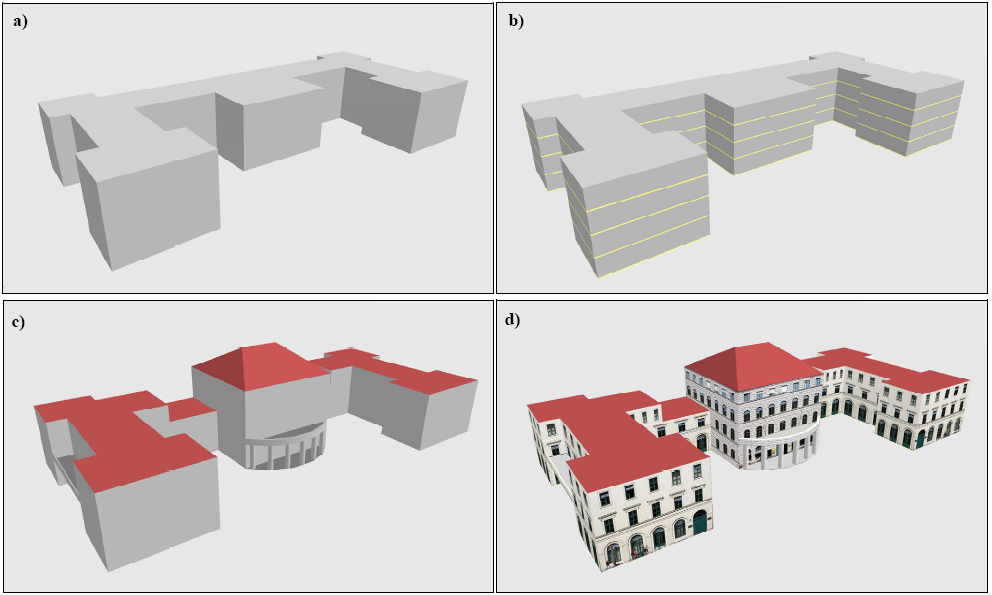
\includegraphics[width=15cm]{gfx/lodcity05-1.png}
	\caption{Continuous LOD: a) block model; b) building split into floors; c) geometry refinement; d) appearance refinement.}
	\label{FIG-LODCITY}
\end{figure}

A building is composed of a list of floor objects. A floor object refers to a floor prototype, which
contains the floor specification. This indirection allows a user to reuse floor prototypes in several
floors of the same building and allows rendering optimizations.

Each floor prototype is defined by its ground plan, which is one or more polygons that define the area
on which walls can be constructed. There can be inner loops in order to allow features like courtyards.
A ground plan supports thickness, useful for defining terraces.

On top of a ground plan one can place walls. A wall represents a vertical, planar polygon.
The default type of wall has no thickness, sufficient if a group of them form a closed surface
and can be only seen from the outside. Thick walls can also be added.
A wall can be lower or higher than its floor height, allowing balcony fronts and chimneys to be defined.

The higher ground plans can have roofs. The most common roof types are supported (hipped, gabled, tent,
mansard, pent, barrel) and a roof is described only by choosing the floor type and placing its
most relevant points (known as the roof skeleton).

Each floor prototype has a related floor decoration. A floor decoration is a collection of facade sections
and window sections. The former allows whole wall sections to be assigned a material while the latter
allows the definition of positioning and appearance of the floor's windows.

TODO: other relevant articles?

\subsection{Getting User Input}
Obtaining user input can happen in an infinity of interface combinations.
In virtual reality the most common solutions may feature:
\begin{itemize}
	\item image processing using camera(s)
	\item speech recognition
	\item motion tracking
	\item space ball, space pilot, etc.
	\item HMD's rotation data
	\item tracked artifacts for direct manipulation
\end{itemize}

The least intrusive interface would use either motion tracking or image processing and speech recognition.
Speech recognition allows commands to be given to the system. The remaining interface allows knowing positioning
and rotation of users or parts of their bodies. Tracking artifacts may either allow the artifact to serve as a
pointer or as a metaphor for direct manipulation.

\subsection{Sketching for Geometry Creation and Editing}

\subsubsection{Smart Sketchpad}
Wenyin et al. created Smart Sketchpad \cite{SMARTSK01}.
Smart Sketchpad recognizes standard shapes (rectangles, triangles, ellipses, straight lines)
and compound shapes such as arrowheads.

Their article describes the steps necessary for shape recognition:
\begin{enumerate}
	\item input as a chain of points
	\item polygonalize to polyline and refine endpoints
	\item close near endpoints - if closed go to step 6
	\item if line ends near another line end, join them and go to step 3
	\item classify line as one of: straight line, polyline or free form curve. go to step 8
	\item close shape recognition *
	\item estimate the parameter of the closed shape
	\item test if shape can be combined with other shapes in the drawing. If so repeat step 8, else end
\end{enumerate}

The $6^{th}$ step was tested with: rule-based system, support vector machine and neural network.
The most successfully approach was SVN, with 97,5\% success, closely followed by NN.

\subsubsection{Assist}
Alvarado and Davis present a work toward an interface for mechanical designers named Assist \cite{FREEDOM01},
with the purpose of allowing them to sketch naturally and have the computer interpreting
their strokes into shapes like rods, hinges, polygons, etc.

The interpretation is a three stages procedure:

\begin{itemize}
	\item match strokes to a series of templates
	\item rank interpretations with several heuristics about drawing style and mechanical engineering
	\item return the most consistent hypothesis
\end{itemize}

Figure \ref{FIG-FREEDOM01} illustrates the result.

The authors emphasize the difficulty they faced when replacing the original human-made stroke
by its computer interpretation. Users prefer composing the whole drawing prior to computer
interpretation replacement. Having the computer interpreting every stroke makes them feel they're
giving up control of the program. Even so, that was the path chosen by the authors because
every extra stroke without giving feedback to the user increases the chance of misinterpretations.
Another relevant conclusion is that users expect symmetry to be kept regarding the interpreted
shapes, so it would be a good idea to detect and suggest alignment restrictions between shapes.

\begin{figure}[htb]
	\centering
	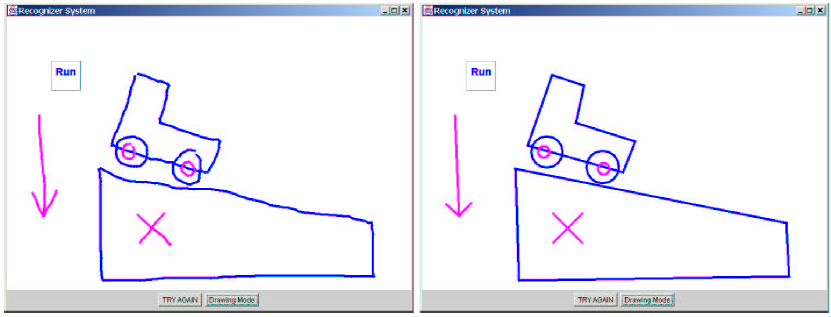
\includegraphics[width=15cm]{gfx/freedom01-1.png}
	\caption{Assist: A car on the hill. Drawn by the user (left), as interpreted and displayed (right).}
	\label{FIG-FREEDOM01}
\end{figure}

\subsubsection{Digital Clay}
Digital Clay \cite{DIGCLAY00} allows a user to draw freely and tries to convert the drawing into a 3D model.
See input and 3D result in Figure \ref{FIG-DIGCLAY}.

It uses two techniques to achieve that:

\begin{itemize}
	\item Huffman-Clowes algorithm, which identifies concave and convex vertices, requiring
	every line to connect to another line and the program additionally demands the object
	drawn to be solid;
	\item infers 3D coordinates based on inherent rules that govern each type of drawing projection.
	Examples: axes of isometric drawings have equal angles between them;
	perspective drawings show foreshortening of lines as we get closer to the viewer.
\end{itemize}

The downfalls of this method are the impossibility of describing occluded faces and the limited
editing capacities available once the conversion has been done.

\begin{figure}[htb]
	\centering
	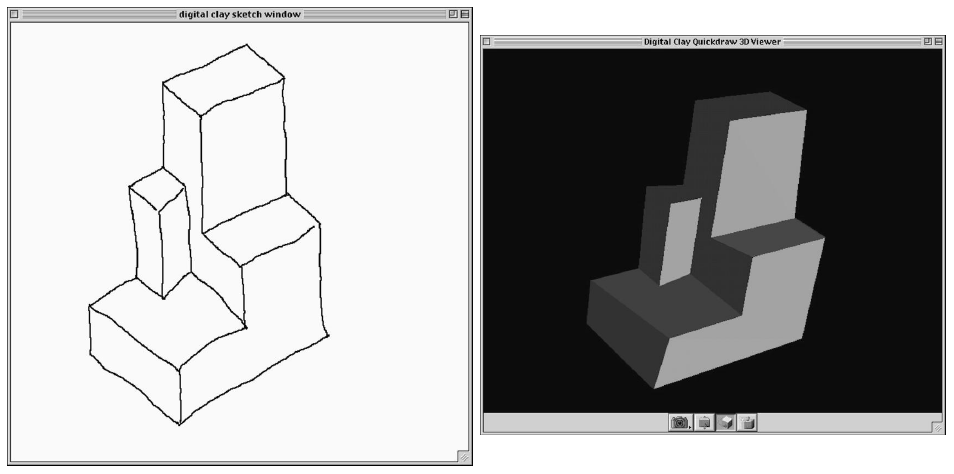
\includegraphics[width=15cm]{gfx/digclay00-1.png}
	\caption{Digital Clay: Raw sketch input and its 3D interpretation.}
	\label{FIG-DIGCLAY}
\end{figure}

\subsubsection{Discussion}

TODO!

\subsection{Helping the User: Suggested Constraints}

\subsubsection{Pegasus}
Igarashi and Hinckley present a 2D sketching system named Pegasus \cite{BEAUTY97}.
It receives user strokes and converts them, generating candidates by taking into account restrictions for:
vertex connection, segment connection, parallelism, perpendicularity,
alignment, congruence, symmetry and interval equality.

The application presents the most relevant candidates to the user and highlights the highest relevant one.
The user can either accept it or select another candidate by tapping on it as seen of Figure \ref{FIG-PEGASUS}.

\begin{figure}[htb]
	\centering
	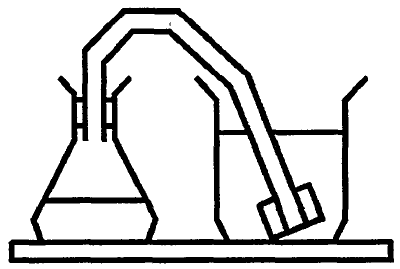
\includegraphics[width=6cm]{gfx/beauty97-1.png}
	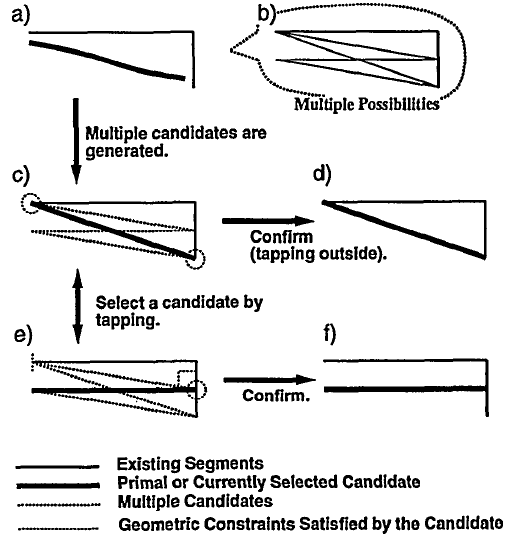
\includegraphics[width=6.5cm]{gfx/beauty97-2.png}
	\caption{Pegasus: A diagram drawn on Pegasus without using any editing commands such as rotation, copy or gridding (left); interaction with multiple candidates (right).}
	\label{FIG-PEGASUS}
\end{figure}

\subsubsection{Discussion}

TODO
%(PEGASUS): The technique appears to be of great use in my project - in architecture most walls subsume these constraints.
%Additionally my users will model in 3D, which increases the interest in applying beautification algorithms
%such as this one.

\subsection{Navigation}

\subsubsection{Smart and Physically Based Navigation}
In order to ensure users not ''getting lost'' in the virtual space, Buchholz, Bohnet and D�llner \cite{SMARTCAM05} propose
a camera that is is both smart and physically-based. Smart in the sense that it is aware of confusing,
disorienting viewing situations and provides means to circumvent them. Physically based because it is
supported by a physically based model of the 3D motion to ensure steady, continuous user movements.

In order to solve the disorientation problem the camera has to identify situations when to intervene. For that
matter a metric, called orientation value, was created. Each view is classified by counting its pixels, granting
different scores: highest values for landmarks; high values for terrain; low values for the sky.
Therefore a threshold can be established and views below it are classified ''disoriented''.

When such an event takes place, smart navigation techniques restrict camera control. The constraints posed
to user control must be as comprehensible as possible. Camera movement should also be time-coherent and physically sound.

The maintenance strategy solves critical situations such as (see Figure \ref{FIG-SMARTCAM1}, left):

\begin{enumerate}[a)]
	\item The user rotates the flight direction and causes the camera to look too far beyond the terrain border.
		The rotation is accepted but outweighed by a slight rear movement away from the border.
	\item The user is flying forward beyond the terrain border.
		The maintenance strategy temporarily tilts down the view direction until a maximum angle is reached.
	\item If no more tilting is possible, the strategy rotates the flight direction parallel to the terrain
		to fly along the terrain border.
\end{enumerate}

\begin{figure}[htb]
	\centering
	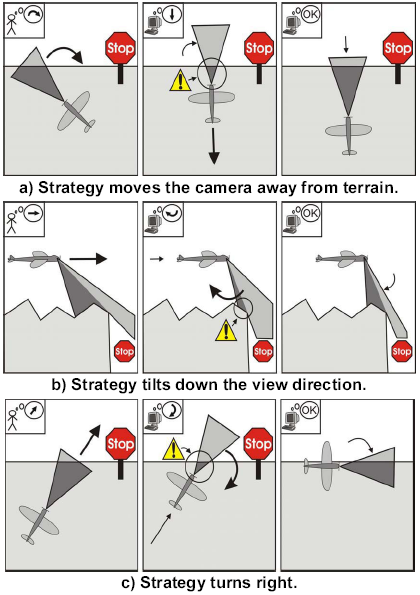
\includegraphics[width=5cm]{gfx/smartcam05-1.png}
	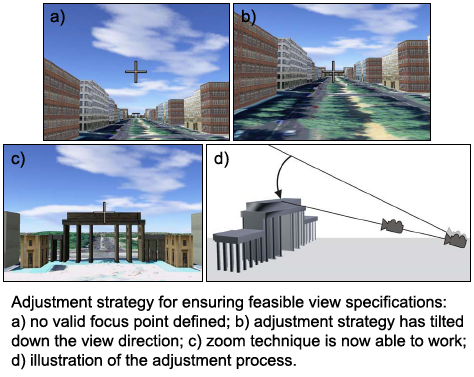
\includegraphics[height=3cm]{gfx/smartcam05-2.png}
	\caption{SPB Cam: Maintenance strategy for keeping high orientation values (left); Adjustment strategy for ensuring of feasible view specifications (right).}
	\label{FIG-SMARTCAM1}
\end{figure}

TODO end article!


%\subsubsection{}

%\cite{SKAN02}
%\cite{DESFUT04}



\newpage

\section{Comparative Analysis}
\TODO{add my ideas for solution}
% comparison table of various solutions
% Analyze and comment solutions
% Add out idea for solution

% summary of section:
In this section we will analyze popular solutions available in the market,
highlighting each solution strenghts and weaknesses.
Later on a table is presented summarizing each solution and relevant features compared, and its
data discused.
The section ends with the author's ideas for an alternative solution.

\subsection{AutoCAD}
AutoCAD is the \emph{de facto} standard software for architecture designs.
It has a steep learning curve (Figure \ref{FIG-AUTOCAD}) but is nevertheless
learned all over the world.

One of its formats, DXF, is widely supported in 3D modelers and engines.
AutoCAD features a powerful language, AutoLisp, which allows advanced users to create scripts for
automating any aspect available in the interface.

This program favors 2D drawing and modeling over real 3D concepts,
but a skillful operator can create every shape necessary to an architectural scenario.
Internally AutoCAD doesn't support any interactive preview of the created designs.

It renders using the Mental Ray\footnote{Mental Ray rendering engine -- http://www.autodesk.com/mentalray}\nocite{SITE-MENTAL} engine.
Animations can be made using camera paths.

\begin{figure}[!ht]
    \centering
    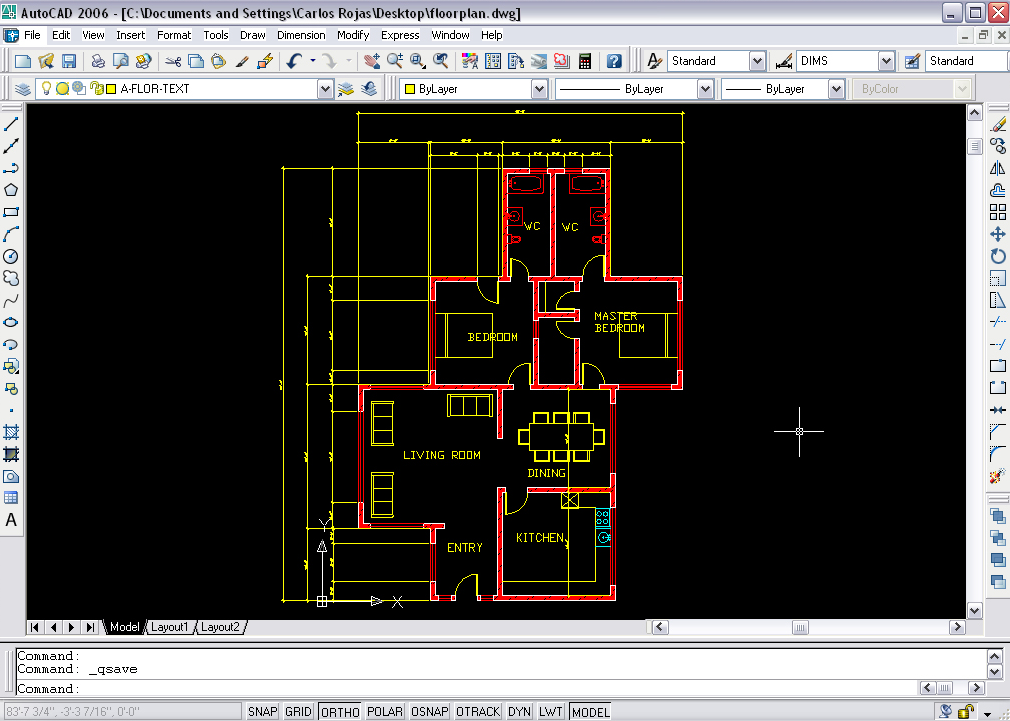
\includegraphics[width=12cm]{gfx/autocad-1.png}
    \caption{AutoCAD: A typical layout of a floor plan.}
    \label{FIG-AUTOCAD}
\end{figure}

\subsection{ArchiCAD}
\nocite{SITE-ARCHICAD}
GraphiSoft ArchiCAD\footnote{GraphiSoft ArchiCAD -- http://www.graphisoft.com/products/archicad}
aims at conquering new architecture students who haven't been exposed to AutoCAD.

It offers pre-made views and document templates for every architectural driven need.
It is by definition a 3D CAD program and it is praised by architects for its easy 3D
manipulation capabilities (Figure \ref{FIG-ARCHICAD}).

The program features templates for common architectural elements.
ArchiCAD has navigation capabilities too, allowing first person perspective navigation of the model.
Its workflow is thought out to make it easy for an architect to do the most common tasks,
making it a friendlier alternative when compared to AutoCAD.
It lacks the expressive power to do about 10\% uncommon tasks though.

There's a Software Development Kit for ArchiCAD plugin creation.

\begin{figure}[!ht]
    \centering
    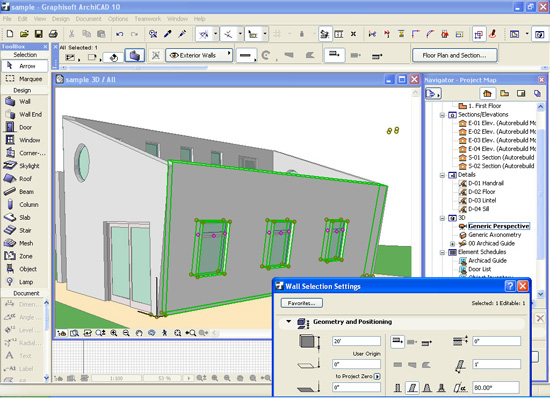
\includegraphics[width=12cm]{gfx/archicad-1.png}
    \caption{ArchiCAD: Notice basic selection and template properties editing in the 3D view.}
    \label{FIG-ARCHICAD}
\end{figure}

\subsection{Revit Building}
\nocite{SITE-REVIT}
Revit Building\footnote{AutoCAD Revit Building -- http://www.autodesk.com/revit}
is another Autodesk product.
Unlike AutoCAD, which spans its use to other areas such as mechanical engineering,
Revit Building was explicitly thought out for architectural design.

It works completely in 3D and has native templates for doors, windows, roofs, etc.
Features the concept of mass, lacking in most packages.
Common constraints are detected. Thick walls can be drawn as lines and solids can
be cut as floors (compare the top-left and bottom right views in Figure \ref{FIG-REVIT}).

Revit Building features powerful templates for complex tasks such as roof design.
It has a simple raytacer and radiosity engine. Cameras can be placed but only for view
rendering, not animation.

Being a system for the professional segment, it has a lower learning curve and provides
tools that allow successful modeling of complex buildings, even for enthusiasts,
something much harder to do in AutoCAD.

\begin{figure}[!ht]
    \centering
    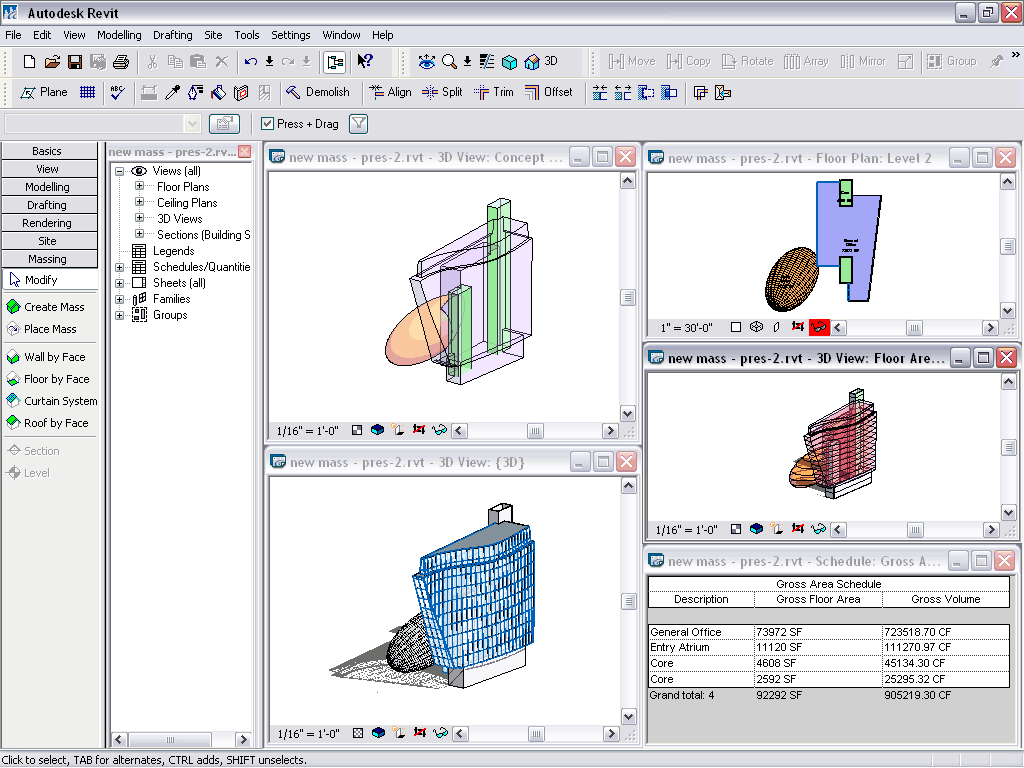
\includegraphics[width=12cm]{gfx/revit-1.png}
    \caption{Revit Building: Solid shapes can be combined with boolean operations and converted into buildings.}
    \label{FIG-REVIT}
\end{figure}

\subsection{SketchUp}
\nocite{SITE-SKETCHUP}
Google SketchUp\footnote{Google SketchUp -- http://www.sketchup.com}
is a friendly program for the novice 3D modeler.
It features a simple interface and most of its tools are basic,
still able to achieve acceptable results.
Its learning curve is great -- everyone can sketch a room in a nick of time.

Its engine is based on drawing lines on top of lines,
already created surfaces or a construction plane.
It detects the most common geometry restrictions (such as midpoint and perpendicularity).

Features an online repository of models, allowing importing of objects such as
furniture, trees, props or well known buildings by just browsing and selection.

Performs strange results when handling awkward angles or when several lines
are the vicinity of the mouse.
Curve manipulation and generation of surfaces is nonexistent.
Allows plugin design in the Ruby language.

Another bonus from being part of the Google software library, SketchUp features import/export capabilities to Google Earth
\footnote{Google Earth -- http://earth.google.com}\nocite{SITE-EARTH}.
This allows capturing a patch of land to SketchUp, design a building there and export the patch
back with its new contents to Google Earth.

A great feature SketchUp is realtime shadows (Figure \ref{FIG-SKETCHUP}) -- since there's only one viewport, shadows are crucial to give the user a sense of depth to a scene.

In renders cartoonish styled views and allows interpolation of cameras to render simple animations.

The professional version of the program allows exporting to common 3D architectural formats.


\begin{figure}[!ht]
    \centering
    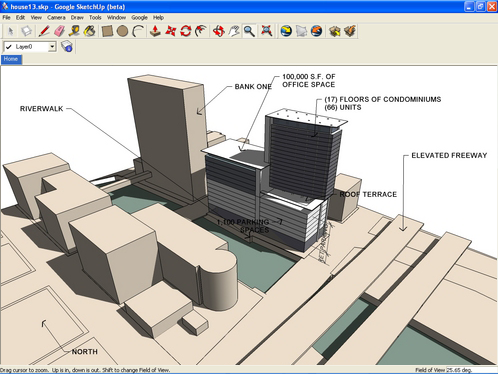
\includegraphics[width=12cm]{gfx/sketchup-1.png}
    \caption{SketchUp: Basic shape extrusions. Notice the shadows in the viewport.}
    \label{FIG-SKETCHUP}
\end{figure}

\newpage

\subsection{Comparison Table of Available Solutions}
\begin{table}[!ht]
    \centering
		\begin{tabular}{|c|c|c|c|c|}
			\hline
			\backslashbox{Features}{Solutions}		& AutoCAD		& ArchiCAD	& Revit Building	& SketchUp	\\
			\hline
			Design in 2D						&		\GdA		&		\GdB		&				\GdB			&		\GdC		\\
			\hline
			Design in 3D						&		\GdD		&		\GdC		&				\GdB			&		\GdB		\\
			\hline
			Architectural Templates	&		\GdD		&		\GdB		&				\GdA			&		\GdC		\\
			\hline
			Supported Formats				&		\GdC		&		\GdC		&				\GdB			&		\GdD / \GdB \footnotemark\\
			\hline
			Interactive Modes				&		\GdE		&		\GdB		&				\GdC 			&		\GdE		\\
			\hline
			Rendering Capabilities	&		\GdB		&		\GdB		&				\GdC			&		\GdD		\\
			\hline
			Extensibility						&		\GdA		&		\GdC		&				\GdE			&		\GdC		\\
			\hline
		\end{tabular}
		\caption{Different solutions in the market compared.}
		\label{TB-COMP-SOL}
\end{table}
\footnotetext{SketchUp exporting capabilities depend on using free or commercial version}

\begin{table}[!ht]
    \centering
		\begin{tabular}{|p{2cm}|p{2cm}|p{2cm}|p{2cm}|p{2cm}|}
			\hline
			very bad	& bad			& average	& good		& very good	\\
			\hline
				\GdE		&	\GdD		&	\GdC		&	\GdB		&	\GdA			\\
			\hline
		\end{tabular}
  \caption{Legend of Table \ref{TB-COMP-SOL}}
  \label{TB-COMP-SOL-LEGEND}
\end{table}

\subsection{Discussing the Table}
AutoCAD makes use of a well established workflow, which takes time to master.
There's a way of doing everything architecturally speaking, though most times a difficult one.
Since its a package general enough for supporting other uses, AutoCAD doesn't come with architectural
templates, a very helpful feature available in both ArchiCAD and Revit Building.

Revit Building is Autodesk's vision of an easy to master, yet powerful system for architectural design.
Revit Building and ArchiCAD are the most similar systems.
Revit Building has better modeling features while ArchiCAD has many document templates
ready for extracting bureaucratic papers out of the architect's workflow.

SketchUp is undoubtfully the most amateur of the analyzed systems.
It offers limited geometrical operations and doesn't have a real template library.
It tries to overcome that limitation by offering a large online repository of models.
SketchUp's best qualities are its learning curve -- any user can feel confident in
modeling a simple floor in a couple of minutes -- and the Google Earth connection.

It would be of great use if other programs were granted permission to get geographical
data (both height maps and texture maps) of an area on Earth.
This offers an important head start for an architect in designing a building that
smoothly blends in its surroundings.


\newpage

\section{Conclusions \& Future Work}
% a summary of the most relevant conclusions that appear throught the document
There is interest in a solution that offers free form sketching for early stages of
design and with good navigational and reviewing capabilities.
The surveyed articles make it clear that it is nowadays feasible to build such a system.
A number of decisions must be made in order to develop such system, both in terms of
main purpose of the system, available hardware and facilities, number of users to serve
simultaneously and the precision vs freedom in sketching.

Multimodal interfaces allow for more successful creative designs by offering a least intrusive
way of controlling the system. Beautification improves user's ability to sketch geometrically.
3D reconstruction can be successfully accomplished for a given domain such as architecture
given a number of guidelines are respected. Suggestive interfaces allow the user to aid the
system in the interpretation task of forms.

The market offers a number of solutions for architecture design.
An evolution can be seen in terms of ease of use and aiding tools offered by the most recent
packages, allowing a less experienced user to feel confident in small architecture tasks.

% directions where to lead efforts in future work


%\onecolumn
\newpage

%\bibliographystyle{plain}
\bibliographystyle{alpha}   % this style uses the authors first letters followed by year
\bibliography{thesis}

\end{document}
